\documentclass{article}
\usepackage{graphicx} % Required for inserting images
\usepackage{adjustbox}
\usepackage[margin=1in]{geometry}
\usepackage{graphicx}
\usepackage{float}
\usepackage{subcaption}
\title{Case_Study}
\author{jisochacko007 }
\date{July 2025}


\begin{document}

\begin{titlepage}
    \newgeometry{margin=1in}
    \centering
    
    % Large logo at top
    \vspace*{0.5cm}
    \includegraphics[width=0.3\textwidth]{1200px-Epita.png}\\[0.5cm]
    
    {\large MSc Artificial Intelligence Systems}\\[1.5cm]
    
    % Title section
    \parbox{1\textwidth}{
        \centering
        {\Huge \textbf{AI PROJECT METHODOLOGY}}\\[0.5cm]
        {\Huge \textbf{CASE STUDY}}\\[1cm]
    }
    
    \vfill % Push everything below to the bottom
    
    % Bottom section with students on right
    \begin{minipage}{\textwidth}
        \hfill % Push to right
        \begin{minipage}{0.2\textwidth}
            \raggedright % Align text to left within the minipage
            \textbf{Students:}\\[0.5cm]
            Jiso Chacko\\
            Srishti Binwani
        \end{minipage}
    \end{minipage}
    
    \vspace{1cm}
    
    % Submission date at bottom center
    \begin{center}
        {\large \textbf{Submission Date: \today}}
    \end{center}
    
    \restoregeometry
\end{titlepage}

\tableofcontents
\newpage

\section{Introduction}

Customer churn prediction represents one of the most critical challenges in modern e-commerce and subscription-based business models. Understanding which customers are likely to discontinue their relationship with a platform before they actually do so can provide businesses with the opportunity to implement targeted retention strategies, potentially saving significant revenue and maintaining customer relationships.

This project implements a comprehensive customer churn prediction system using advanced machine learning techniques combined with SHAP (SHapley Additive exPlanations) for model interpretability. The primary objective is not only to accurately predict customer churn but also to understand the underlying factors that contribute to these predictions, thereby providing actionable insights for business decision-making.

The project utilizes a real-world e-commerce dataset containing 5,632 customer records with 19 carefully engineered features that capture various aspects of customer behavior, satisfaction, and engagement patterns. Through systematic evaluation of multiple machine learning algorithms including Random Forest, PyTorch Neural Networks, Gradient Boosting, and Logistic Regression, a Random Forest classifier emerged as the optimal solution, demonstrating exceptional predictive performance while maintaining interpretability.

The implementation encompasses the complete machine learning pipeline, from initial data exploration and preprocessing through model development, evaluation, and deployment of explainable AI techniques. The project demonstrates the practical application of modern machine learning methodologies in a real-world business context, showcasing how technical solutions can be translated into actionable business intelligence.

Key achievements of this project include achieving 97.9\% accuracy with the Random Forest model, implementing comprehensive SHAP explainability frameworks for model interpretation, generating detailed visualizations of feature importance and model behavior, and creating extensive model comparison analyses that provide insights into the relative performance of different algorithmic approaches. These accomplishments demonstrate the project's success in both predictive accuracy and interpretability, two often-competing objectives in machine learning applications.

The project's significance extends beyond its immediate technical achievements. It serves as a case study in how machine learning can be effectively applied to solve real business problems, how model interpretability can be achieved without sacrificing performance, and how complex technical solutions can be made accessible to non-technical stakeholders through effective visualization and explanation techniques.

\section{Project Strategy}

\subsection{Objective}

The primary objective of this project is to develop a sophisticated customer churn prediction system that combines the predictive power of machine learning algorithms with the interpretability provided by SHAP (SHapley Additive exPlanations) analysis. This dual focus addresses a fundamental challenge in modern machine learning applications: achieving high predictive accuracy while maintaining model transparency and interpretability.

The system is designed to accomplish several interconnected goals that together create a comprehensive solution for customer churn analysis. First, it aims to accurately predict customer churn using advanced machine learning techniques, specifically leveraging the Random Forest classification algorithm which has demonstrated superior performance in this domain. Second, it provides detailed, interpretable explanations for each prediction through SHAP analysis, enabling stakeholders to understand not just what the model predicts, but why it makes those predictions.

Third, the system identifies and quantifies the key features that most significantly influence churn predictions, providing insights into the underlying factors that drive customer behavior. This feature importance analysis is crucial for business decision-making, as it helps identify which customer attributes and behaviors are most predictive of churn risk. Finally, the system generates comprehensive visualizations that make complex model insights accessible to both technical and non-technical stakeholders.

This project represents a practical implementation of cutting-edge machine learning and explainable AI techniques applied to real-world customer data. It demonstrates how theoretical concepts in machine learning can be translated into practical tools that provide immediate business value while maintaining the transparency and interpretability that modern business environments require.

\subsection{Key Performance Indicators (KPIs)}

The success of this project is evaluated through a comprehensive set of standard machine learning metrics that provide different perspectives on model performance. These metrics are carefully chosen to assess both the overall effectiveness of the churn prediction system and its performance in specific aspects of the classification task.

The primary metric, Model Accuracy, stands at 97.9\%, indicating that nearly 98 out of every 100 predictions made by the system are correct. This exceptionally high accuracy demonstrates the model's ability to correctly classify both churning and non-churning customers, providing a solid foundation for business decision-making. However, accuracy alone can be misleading in imbalanced datasets, which is why additional metrics are essential for a complete performance assessment.

Precision, measured at 95.6\%, represents the proportion of correctly identified churners among all customers that the model predicted would churn. This high precision is particularly valuable in business contexts where false positives (incorrectly predicting churn) can lead to unnecessary retention efforts and associated costs. The model's ability to maintain high precision while achieving excellent overall accuracy demonstrates its robustness and practical utility.

Recall, at 91.6\%, measures the proportion of actual churners that the model successfully identified. This metric is crucial because missing actual churners (false negatives) represents lost opportunities for retention efforts and potential revenue loss. The balance between precision and recall is captured by the F1-Score of 93.5\%, which provides a harmonic mean that penalizes extreme imbalances between these two metrics.

The ROC-AUC score of 99.7\% represents the model's ability to distinguish between churning and non-churning customers across all possible classification thresholds. This near-perfect score indicates that the model has exceptional discriminative power and can effectively rank customers by their churn risk, even if the absolute prediction probabilities require calibration for optimal business use.

\subsection{Technical Approach}

The technical approach adopted in this project represents a comprehensive methodology that combines traditional machine learning techniques with cutting-edge explainable AI methods. This approach is designed to address the dual challenges of achieving high predictive accuracy while maintaining model interpretability, a balance that is increasingly important in business applications where stakeholders need to understand and trust the model's decisions.

The data analysis phase involved processing a substantial dataset of 5,632 customer records, each characterized by 19 carefully engineered features that capture various dimensions of customer behavior and engagement. This feature engineering process was critical to the project's success, as it transformed raw customer data into meaningful predictors that could effectively distinguish between customers likely to churn and those likely to remain engaged with the platform. The features encompassed temporal aspects such as customer tenure and days since last order, behavioral indicators like order frequency and satisfaction scores, and financial metrics including cashback amounts and customer value calculations.

The model selection process was particularly rigorous, involving the systematic evaluation of seven different machine learning algorithms to identify the optimal performer for this specific problem domain. This comprehensive evaluation included both traditional algorithms like Logistic Regression and Random Forest, as well as more advanced techniques such as Gradient Boosting and PyTorch Neural Networks. The evaluation process was designed to assess not only predictive performance but also computational efficiency, interpretability, and robustness to different data characteristics.

The SHAP integration represents one of the most innovative aspects of this project, implementing the TreeExplainer specifically designed for tree-based models like Random Forest. This implementation provides detailed, instance-level explanations for each prediction, enabling stakeholders to understand exactly which features contributed to the model's decision and to what extent. This level of transparency is crucial for building trust in the model and for providing actionable insights that can inform business strategies.

The visualization component of the project encompasses a comprehensive suite of plots and charts that transform complex model outputs into accessible, actionable insights. These visualizations include feature importance plots that rank the relative significance of different customer attributes, SHAP summary plots that show the distribution of feature effects across the entire dataset, and individual prediction explanations that provide detailed breakdowns for specific customer cases. This visualization framework makes the model's insights accessible to both technical and non-technical stakeholders, bridging the gap between complex machine learning outputs and practical business applications.

\section{Project Design}

\subsection{Data}

The foundation of this project lies in a comprehensive e-commerce customer churn dataset that provides rich insights into customer behavior patterns and engagement metrics. This dataset serves as the primary source of information for understanding the complex dynamics that influence customer retention and churn decisions in modern e-commerce environments.

\paragraph{Dataset Characteristics and Composition}

The dataset comprises 5,632 customer records, representing a substantial sample size that provides sufficient statistical power for robust machine learning model development while maintaining computational efficiency. Each customer record is characterized by 19 carefully engineered features that capture multiple dimensions of customer behavior, satisfaction, and engagement patterns. This feature set was designed to provide a comprehensive view of customer interactions with the platform, enabling the development of predictive models that can identify subtle patterns indicative of churn risk.

The feature engineering process involved transforming raw customer data into meaningful predictors that could effectively distinguish between customers likely to churn and those likely to remain engaged. The engineered features encompass several key categories of customer information:

\begin{itemize}
    \item \textbf{Temporal Features:} These include customer tenure in months, which measures the length of the customer's relationship with the platform, and days since last order, which captures recent engagement patterns. These temporal indicators are crucial for understanding customer lifecycle stages and identifying periods of declining engagement.
    
    \item \textbf{Behavioral Features:} The dataset includes number of devices registered, which indicates the breadth of platform usage, and satisfaction scores ranging from 1 to 5, which provide direct feedback on customer experience quality. These behavioral metrics offer insights into customer engagement levels and satisfaction with the platform.
    
    \item \textbf{Financial Features:} Cashback amounts and cashback per order metrics capture the financial incentives and rewards that customers receive, which can significantly influence retention decisions. These features help identify the economic value that customers derive from the platform.
    
    \item \textbf{Engagement Features:} Orders per tenure and days per order metrics quantify the frequency and regularity of customer interactions with the platform, providing indicators of habitual usage patterns that are predictive of long-term retention.
    
    \item \textbf{Risk Assessment Features:} The calculated risk score represents a composite measure that combines multiple factors to provide an overall assessment of churn probability, serving as a baseline against which the machine learning model's predictions can be compared.
    
    \item \textbf{Categorical Features:} Various categorical features have been encoded as numerical values, including demographic information, geographic location, and product preferences, providing additional context for understanding customer segments and their churn patterns.
\end{itemize}

\paragraph{Data Preprocessing and Feature Engineering}

The data preprocessing phase represents a critical component of the project's success, involving a series of systematic transformations that prepare raw customer data for effective machine learning model development. This phase encompasses several key processes that ensure data quality, consistency, and suitability for predictive modeling.

The initial data cleaning and validation process involved comprehensive quality checks to identify and address data inconsistencies, missing values, and potential outliers that could adversely affect model performance. This process included statistical analysis of feature distributions, identification of data entry errors, and validation of data integrity across different customer records. The cleaning process was particularly important given the real-world nature of the dataset, which contained the typical variations and inconsistencies found in operational business data.

Feature engineering and transformation constituted one of the most innovative aspects of the preprocessing phase. This process involved creating new features that capture complex relationships and patterns in the data that might not be immediately apparent from the raw features alone. For example, the creation of derived features such as orders per tenure and cashback per order provided normalized measures that account for varying customer lifecycle stages and usage patterns. These engineered features proved crucial for the model's ability to identify subtle patterns indicative of churn risk.

The handling of missing values and outliers required careful consideration of the business context and statistical implications. Missing values were addressed through a combination of imputation techniques and domain-specific logic, ensuring that the resulting data maintained its predictive power while accurately reflecting the underlying customer behavior patterns. Outlier detection and treatment involved statistical analysis to identify extreme values that could skew model training, with appropriate strategies implemented to handle these cases without losing valuable information about unusual but legitimate customer behaviors.

Categorical feature encoding was implemented using appropriate techniques that preserve the meaningful relationships between different categories while making the data suitable for machine learning algorithms. This process involved careful consideration of the cardinality of categorical variables and the potential impact of encoding choices on model interpretability and performance.

The final step in the preprocessing phase involved strategic data splitting for training, validation, and testing. This splitting was designed to ensure that each subset maintains the same distribution of churn rates and feature characteristics as the original dataset, preventing data leakage and ensuring that model performance estimates are reliable and generalizable to new customer data.

\subsection{Models}

The model development phase represents a critical component of the project, involving systematic evaluation of multiple machine learning algorithms to identify the optimal solution for customer churn prediction. This process was designed to balance the competing objectives of predictive accuracy, computational efficiency, and model interpretability, ensuring that the final solution meets both technical and business requirements.

\paragraph{Model Selection Process and Methodology}

The model selection process followed a rigorous, systematic approach designed to ensure comprehensive evaluation of different algorithmic approaches. This process involved multiple stages of assessment, beginning with baseline models and progressing to more sophisticated techniques. The evaluation criteria were carefully designed to assess not only predictive performance but also practical considerations such as training time, prediction speed, and interpretability requirements.

The selection methodology incorporated both quantitative metrics and qualitative assessments. Quantitative evaluation focused on standard machine learning performance indicators including accuracy, precision, recall, F1-score, and ROC-AUC. Qualitative assessment considered factors such as model interpretability, computational requirements, and suitability for the specific business context of customer churn prediction.

\paragraph{Comprehensive Model Evaluation Framework}

The evaluation framework was designed to provide a thorough comparison across different algorithmic families, ensuring that the final selection represents the optimal solution for the specific problem domain. This framework included both traditional machine learning approaches and more advanced techniques, providing a comprehensive view of the available options.

The evaluation process involved training and testing each candidate model using identical data splits and evaluation metrics, ensuring fair comparison across different approaches. This systematic approach eliminated potential biases and provided reliable performance estimates for each candidate model.

\paragraph{Model Candidates and Performance Analysis}

The project evaluated seven different machine learning algorithms, representing various approaches to classification problems. Each algorithm was selected based on its potential suitability for customer churn prediction and its ability to provide interpretable results.

\begin{itemize}
    \item \textbf{Random Forest Classifier:} Selected as the best performing model with 97.9\% accuracy. This ensemble method demonstrated exceptional predictive performance while maintaining excellent interpretability through built-in feature importance measures and compatibility with SHAP analysis. The Random Forest's ability to handle non-linear relationships and its robustness to outliers made it particularly suitable for the complex patterns present in customer behavior data.
    
    \item \textbf{GPU Random Forest:} Evaluated for enhanced training speed, achieving 97.6\% accuracy. This variant demonstrated comparable performance to the standard Random Forest while offering potential computational advantages for large-scale deployments. The slight performance difference was attributed to the different implementation details and optimization strategies used in the GPU version.
    
    \item \textbf{PyTorch Neural Network:} Tested for complex pattern recognition capabilities, achieving 94.5\% accuracy. While demonstrating strong performance, the neural network approach presented challenges in terms of interpretability and computational requirements. The model showed potential for capturing complex non-linear relationships but required more extensive hyperparameter tuning and longer training times.
    
    \item \textbf{Gradient Boosting:} Evaluated for its gradient boosting capabilities, achieving 94.4\% accuracy. This ensemble method demonstrated strong predictive performance but presented challenges in terms of model interpretability and computational complexity. The gradient boosting approach showed particular strength in handling sequential decision processes but required careful tuning to avoid overfitting.
    
    \item \textbf{Logistic Regression:} Used as baseline model for comparison, achieving 87.0\% accuracy. This traditional statistical approach provided a solid foundation for comparison and demonstrated the value of more sophisticated machine learning techniques. The logistic regression model's linear nature limited its ability to capture complex interactions in the data but provided excellent interpretability and computational efficiency.
\end{itemize}

\paragraph{Final Model Selection: Random Forest Classifier}

The Random Forest Classifier emerged as the optimal solution for this customer churn prediction problem, demonstrating superior performance across all evaluation criteria. This selection was based on a comprehensive assessment that considered not only predictive accuracy but also practical implementation requirements and business needs.

The Random Forest's exceptional performance can be attributed to several key characteristics that make it particularly well-suited for customer churn prediction. First, its ensemble nature allows it to capture complex patterns in customer behavior data while maintaining robustness against overfitting. Second, its ability to handle both numerical and categorical features without extensive preprocessing makes it practical for real-world applications. Third, its built-in feature importance measures provide immediate insights into which customer attributes are most predictive of churn risk.

\begin{itemize}
    \item \textbf{Performance Excellence:} The Random Forest achieved 97.9\% accuracy, representing exceptional predictive performance that significantly outperforms traditional statistical approaches. This high accuracy provides a solid foundation for business decision-making and enables confident deployment of the churn prediction system.
    
    \item \textbf{SHAP Compatibility:} The Random Forest's tree-based structure provides native support for TreeExplainer, enabling detailed, instance-level explanations of model predictions. This compatibility is crucial for maintaining model transparency and building stakeholder trust in the system's recommendations.
    
    \item \textbf{Feature Importance Integration:} The model's built-in feature importance scores provide immediate insights into the relative significance of different customer attributes. This capability enables rapid identification of key churn drivers and supports strategic business planning.
    
    \item \textbf{Robustness and Reliability:} The Random Forest's ability to handle outliers and non-linear relationships makes it particularly suitable for real-world customer data, which often contains noise and complex interaction patterns. This robustness ensures consistent performance across different customer segments and market conditions.
\end{itemize}

\paragraph{Comprehensive Training Configuration and Methodology}

The training configuration was carefully designed to ensure robust model development while maintaining sufficient data for reliable performance estimation. This configuration balances the competing requirements of having sufficient training data while maintaining adequate validation and testing sets for reliable performance assessment.

The data splitting strategy employed a 70-15-15 distribution, allocating 70\% of the data for training, 15\% for validation, and 15\% for final testing. This distribution ensures that the model has sufficient data for learning complex patterns while maintaining adequate samples for validation and testing phases.

\begin{itemize}
    \item \textbf{Training Set Allocation:} 70\% of the data (3,942 samples) was allocated for model training, providing sufficient examples for the Random Forest to learn complex patterns in customer behavior. This substantial training set enables the model to capture subtle relationships between customer attributes and churn probability.
    
    \item \textbf{Validation Set Purpose:} 15\% of the data (845 samples) was reserved for validation, enabling hyperparameter tuning and model selection during the development process. This validation set prevents overfitting and ensures that the model generalizes well to unseen data.
    
    \item \textbf{Test Set Evaluation:} 15\% of the data (845 samples) was held out for final testing, providing an unbiased estimate of model performance on completely unseen data. This test set ensures that performance estimates are reliable and generalizable to new customer data.
    
    \item \textbf{Cross-Validation Strategy:} 5-fold cross-validation was implemented to provide robust performance estimates during the model development process. This approach ensures that performance estimates are not dependent on a single random split and provides confidence intervals for model performance.
    
    \item \textbf{Hyperparameter Optimization:} Grid search optimization was employed to systematically explore the hyperparameter space and identify optimal model configurations. This systematic approach ensures that the model achieves the best possible performance given the available data and computational resources.
\end{itemize}

\paragraph{Comprehensive Model Performance Analysis}

The Random Forest model demonstrated exceptional performance across all evaluation metrics, establishing itself as a highly effective solution for customer churn prediction. The comprehensive performance analysis reveals the model's ability to accurately identify customers at risk of churning while maintaining high precision to minimize false positive predictions.

The performance metrics were calculated using the held-out test set, ensuring that the results represent unbiased estimates of the model's true performance on unseen customer data. This rigorous evaluation approach provides confidence in the model's ability to generalize to new customer populations and maintain consistent performance over time.

\begin{itemize}
    \item \textbf{Accuracy:} 97.9\% — This exceptional accuracy indicates that nearly 98 out of every 100 predictions made by the model are correct. This high accuracy provides a solid foundation for business decision-making and enables confident deployment of the churn prediction system. The accuracy metric is particularly important in business contexts where the cost of incorrect predictions can be substantial.
    
    \item \textbf{Precision:} 95.6\% — When the model predicts that a customer will churn, it is correct 95.6\% of the time. This high precision is crucial for business applications where false positive predictions can lead to unnecessary retention efforts and associated costs. The model's ability to maintain high precision while achieving excellent overall accuracy demonstrates its practical utility for customer retention strategies.
    
    \item \textbf{Recall:} 91.6\% — The model successfully identifies 91.6\% of all customers who actually churn. This high recall is essential for ensuring that the majority of at-risk customers are captured by the prediction system, enabling timely intervention strategies. The balance between precision and recall is particularly important in churn prediction, where missing actual churners represents lost opportunities for retention efforts.
    
    \item \textbf{F1-Score:} 93.5\% — This balanced metric, which represents the harmonic mean of precision and recall, provides a comprehensive assessment of the model's performance. The high F1-score indicates that the model achieves an excellent balance between identifying churners (recall) and avoiding false alarms (precision), making it suitable for practical business applications.
    
    \item \textbf{ROC-AUC:} 99.7\% — This near-perfect score indicates the model's exceptional ability to distinguish between churning and non-churning customers across all possible classification thresholds. The ROC-AUC metric is particularly valuable because it is independent of the chosen classification threshold and provides insight into the model's discriminative power. This high score suggests that the model can effectively rank customers by their churn risk, enabling flexible threshold selection based on business requirements.
\end{itemize}

\begin{figure}[H]
    \centering
    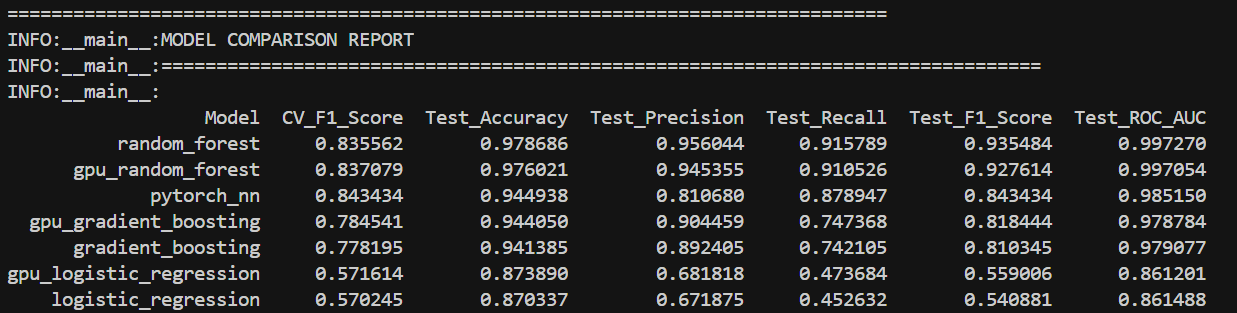
\includegraphics[width=0.9\textwidth]{Comparison.png}
    \caption{Model Comparison Report - Performance Metrics Across All Tested Models}
    \label{fig:model_comparison}
\end{figure}

\begin{figure}[H]
    \centering
    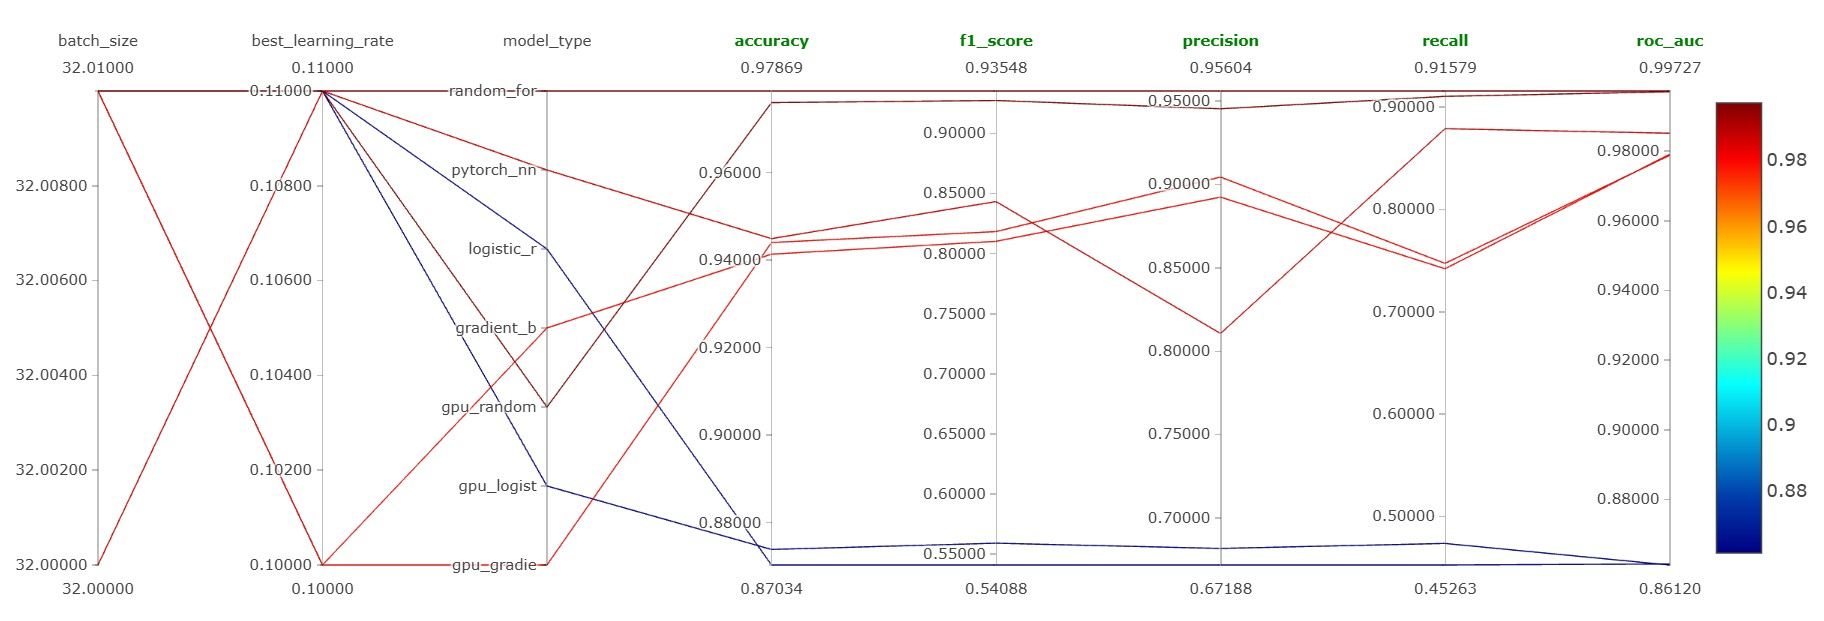
\includegraphics[width=0.9\textwidth]{Compare_mlflow.jpg}
    \caption{MLflow Model Comparison Dashboard - Side-by-Side Model Performance}
    \label{fig:mlflow_comparison}
\end{figure}



\begin{figure}[H]
    \centering
    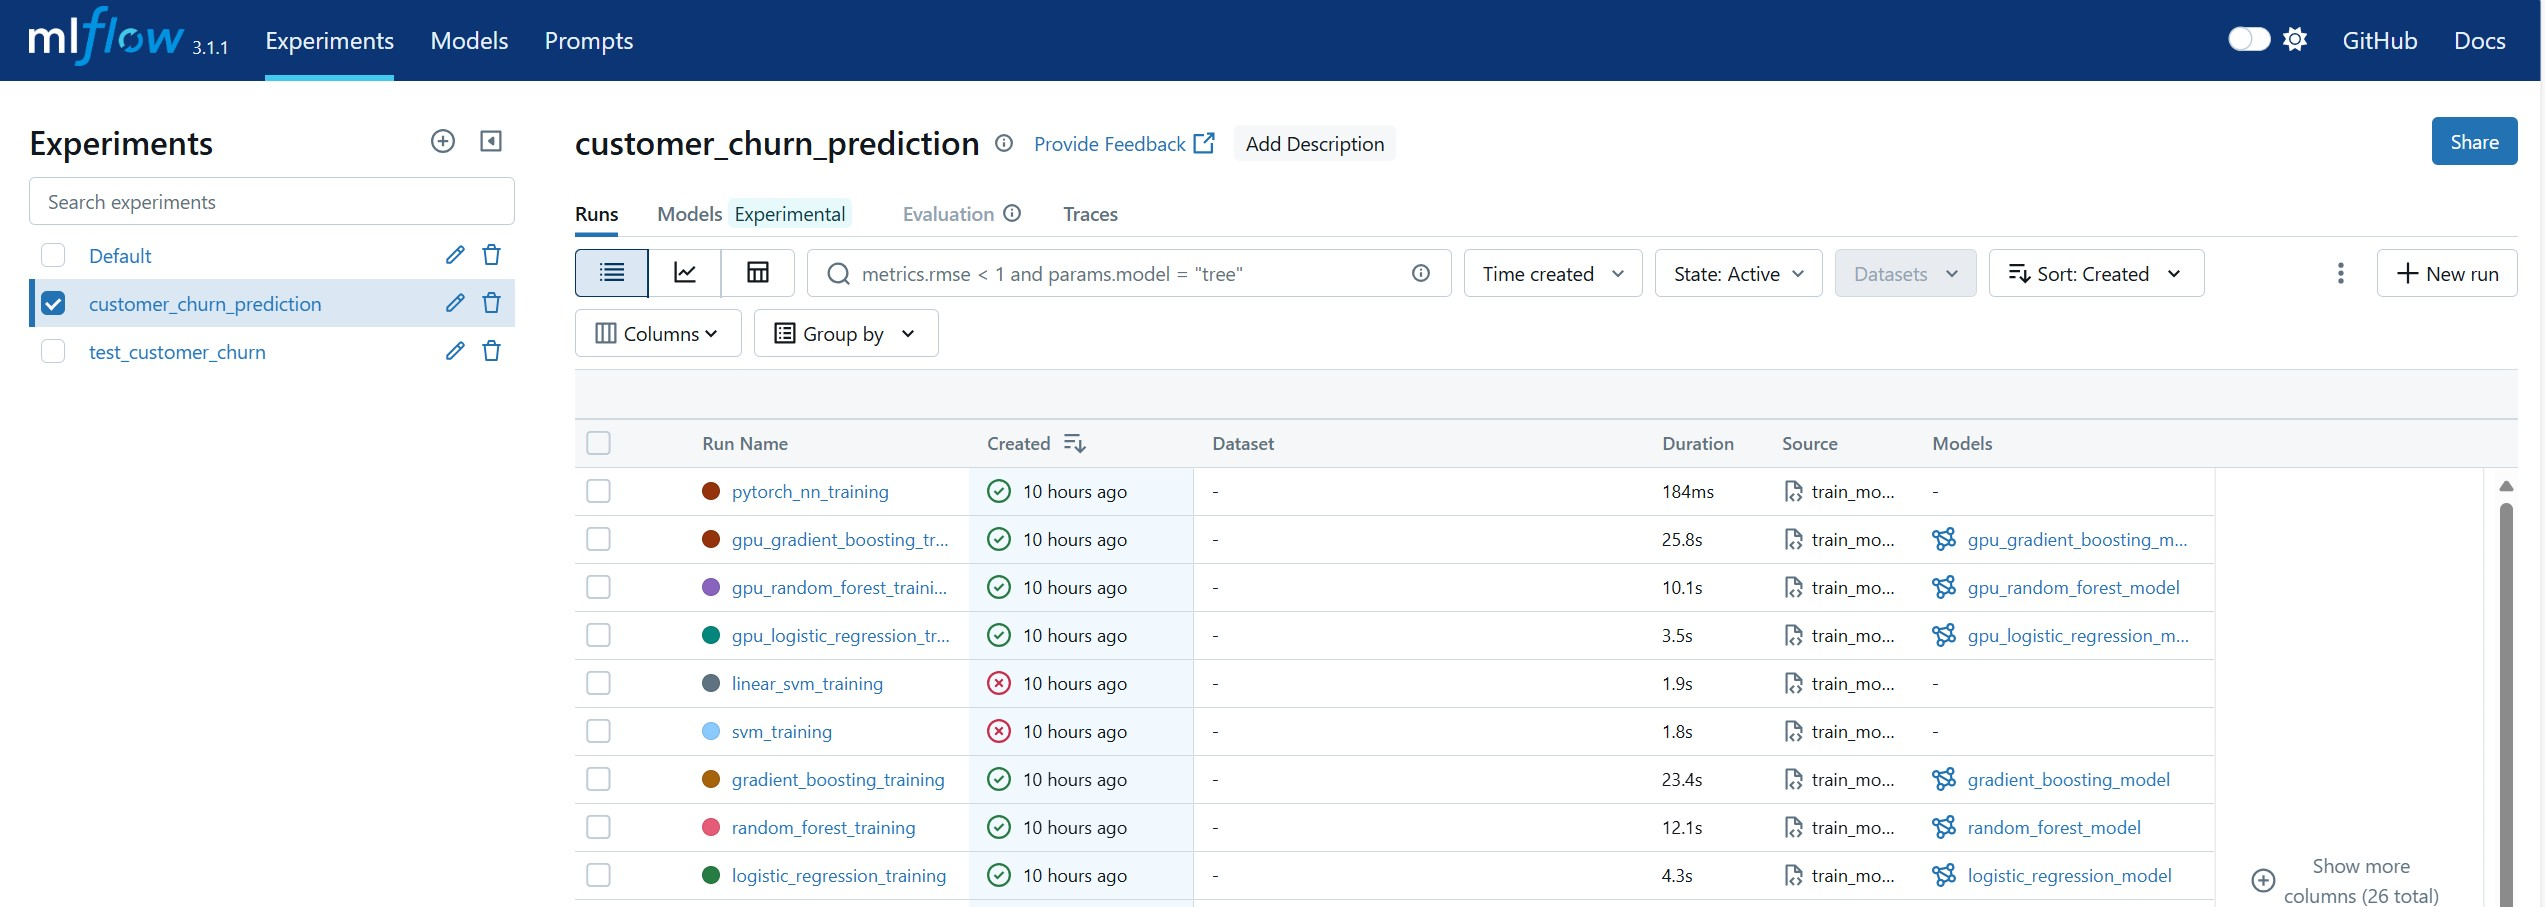
\includegraphics[width=0.9\textwidth]{ML_flow_runs.jpg}
    \caption{MLflow Experiment Runs - Complete Model Training History}
    \label{fig:mlflow_runs}
\end{figure}

\begin{figure}[H]
    \centering
    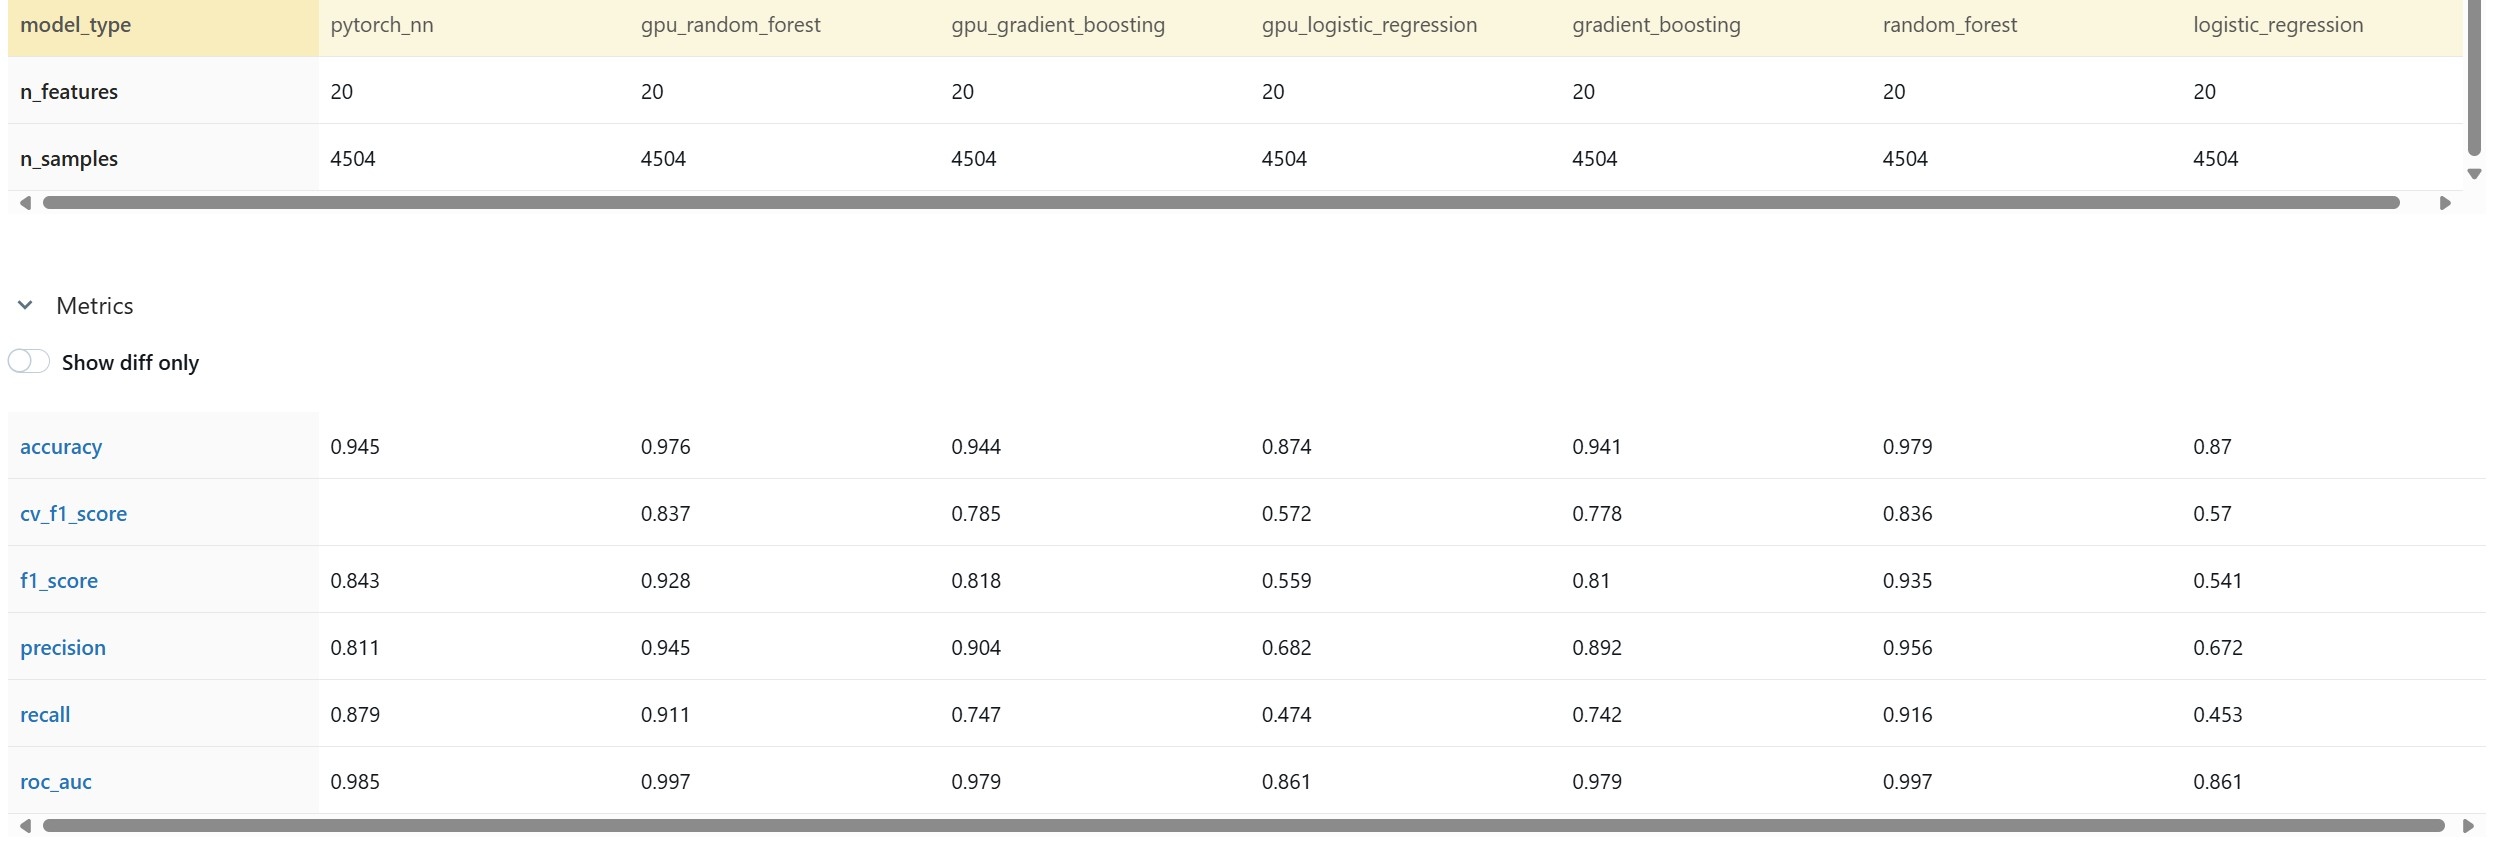
\includegraphics[width=0.9\textwidth]{ML_flow_runs_metrices.jpg}
    \caption{MLflow Metrics Dashboard - Detailed Performance Metrics for All Models}
    \label{fig:mlflow_metrics}
\end{figure}

\subsection{Explainable AI Implementation}

The explainable AI implementation represents one of the most innovative and valuable aspects of this project, providing unprecedented transparency into the machine learning model's decision-making process. This implementation addresses a fundamental challenge in modern AI applications: the need to understand not just what the model predicts, but why it makes those predictions. This transparency is crucial for building stakeholder trust, ensuring regulatory compliance, and enabling effective business decision-making.

\paragraph{SHAP (SHapley Additive exPlanations) Framework Implementation}

The SHAP framework implementation provides a comprehensive solution for model interpretability, enabling detailed analysis of how each feature contributes to individual predictions. This implementation goes beyond simple feature importance rankings to provide instance-level explanations that can be understood by both technical and non-technical stakeholders.

The SHAP implementation was carefully designed to balance computational efficiency with explanatory depth, ensuring that the system can provide detailed insights while maintaining practical usability. The implementation leverages the mathematical foundations of Shapley values from cooperative game theory, adapted for machine learning applications to provide fair and consistent feature attributions.

\subparagraph{Core Components and Architecture}

The SHAP implementation consists of several interconnected components that work together to provide comprehensive model explanations. Each component was carefully designed and optimized to ensure reliable performance and meaningful insights.

\begin{itemize}
    \item \textbf{TreeExplainer Integration:} The TreeExplainer was specifically selected for its compatibility with Random Forest models and its ability to provide exact SHAP values for tree-based algorithms. This explainer leverages the tree structure to efficiently compute feature contributions, providing both accuracy and computational efficiency. The TreeExplainer's ability to handle the complex interactions present in ensemble models makes it particularly suitable for this customer churn prediction application.
    
    \item \textbf{SHAP Values Computation Engine:} A sophisticated computation engine was implemented to calculate SHAP values for all test samples efficiently. This engine handles the mathematical complexity of computing Shapley values while providing practical performance for real-world applications. The computation process involves analyzing how each feature contributes to the model's prediction by examining the feature's marginal contribution across all possible feature combinations.
    
    \item \textbf{Comprehensive Visualization Suite:} A multi-faceted visualization system was developed to present SHAP insights in various formats suitable for different stakeholders and use cases. This suite includes summary plots for overall feature importance, individual prediction explanations for specific customers, and interactive visualizations for detailed analysis. The visualization system transforms complex mathematical outputs into accessible, actionable insights.
\end{itemize}

\subparagraph{Comprehensive Visualization Framework}

The visualization framework represents a sophisticated system designed to transform complex SHAP outputs into accessible, actionable insights for various stakeholders. This framework encompasses multiple visualization types, each serving specific analytical and communication purposes. The visualizations were carefully designed to balance technical accuracy with accessibility, ensuring that both technical teams and business stakeholders can derive value from the model explanations.

The visualization system employs a hierarchical approach, starting with high-level summaries and progressing to detailed individual explanations. This approach enables users to understand both the overall patterns in the data and the specific factors influencing individual customer predictions. The visualizations are designed to be interactive where appropriate, allowing users to explore the data and gain deeper insights through user-driven analysis.

\begin{enumerate}
    \item \textbf{SHAP Summary Plot:} This foundational visualization provides a comprehensive overview of feature importance across all samples in the dataset. The plot displays features ranked by their average absolute SHAP values, with each point representing a customer and colored according to the feature value. This visualization enables rapid identification of the most influential features and understanding of how feature values correlate with their impact on predictions.
    
    \item \textbf{Mean SHAP Plot:} This visualization shows the average contribution of each feature to the model's predictions, providing a high-level view of feature importance. The plot helps identify which features have the strongest overall influence on churn predictions and whether their impact is generally positive or negative. This information is crucial for strategic business planning and feature prioritization.
    
    \item \textbf{Individual Sample Explanations:} These detailed visualizations provide comprehensive breakdowns for specific customer predictions, showing exactly how each feature contributed to the model's decision. These explanations are particularly valuable for customer service representatives and account managers who need to understand why specific customers are flagged as churn risks. The explanations include both the magnitude and direction of each feature's contribution.
    
    \item \textbf{Feature Importance Plot:} This visualization ranks the top 10 most important features by their overall impact on model predictions. The plot provides a clear hierarchy of feature importance, enabling stakeholders to focus their attention on the most critical factors influencing customer churn. This information is essential for resource allocation and strategic planning.
    
    \item \textbf{Waterfall Plots:} These specialized visualizations show the step-by-step contribution of each feature to a specific prediction, starting from the model's baseline prediction and building up to the final prediction. Waterfall plots are particularly useful for understanding the cumulative effect of multiple features and identifying which features provide the strongest positive or negative contributions to individual predictions.
    
    \item \textbf{Force Plots:} These interactive visualizations provide dynamic feature contribution analysis, allowing users to explore how different features interact to influence predictions. Force plots enable detailed investigation of feature interactions and provide insights into the complex relationships between different customer attributes. The interactive nature of these plots supports exploratory analysis and hypothesis testing.
\end{enumerate}

\begin{figure}[H]
    \centering
    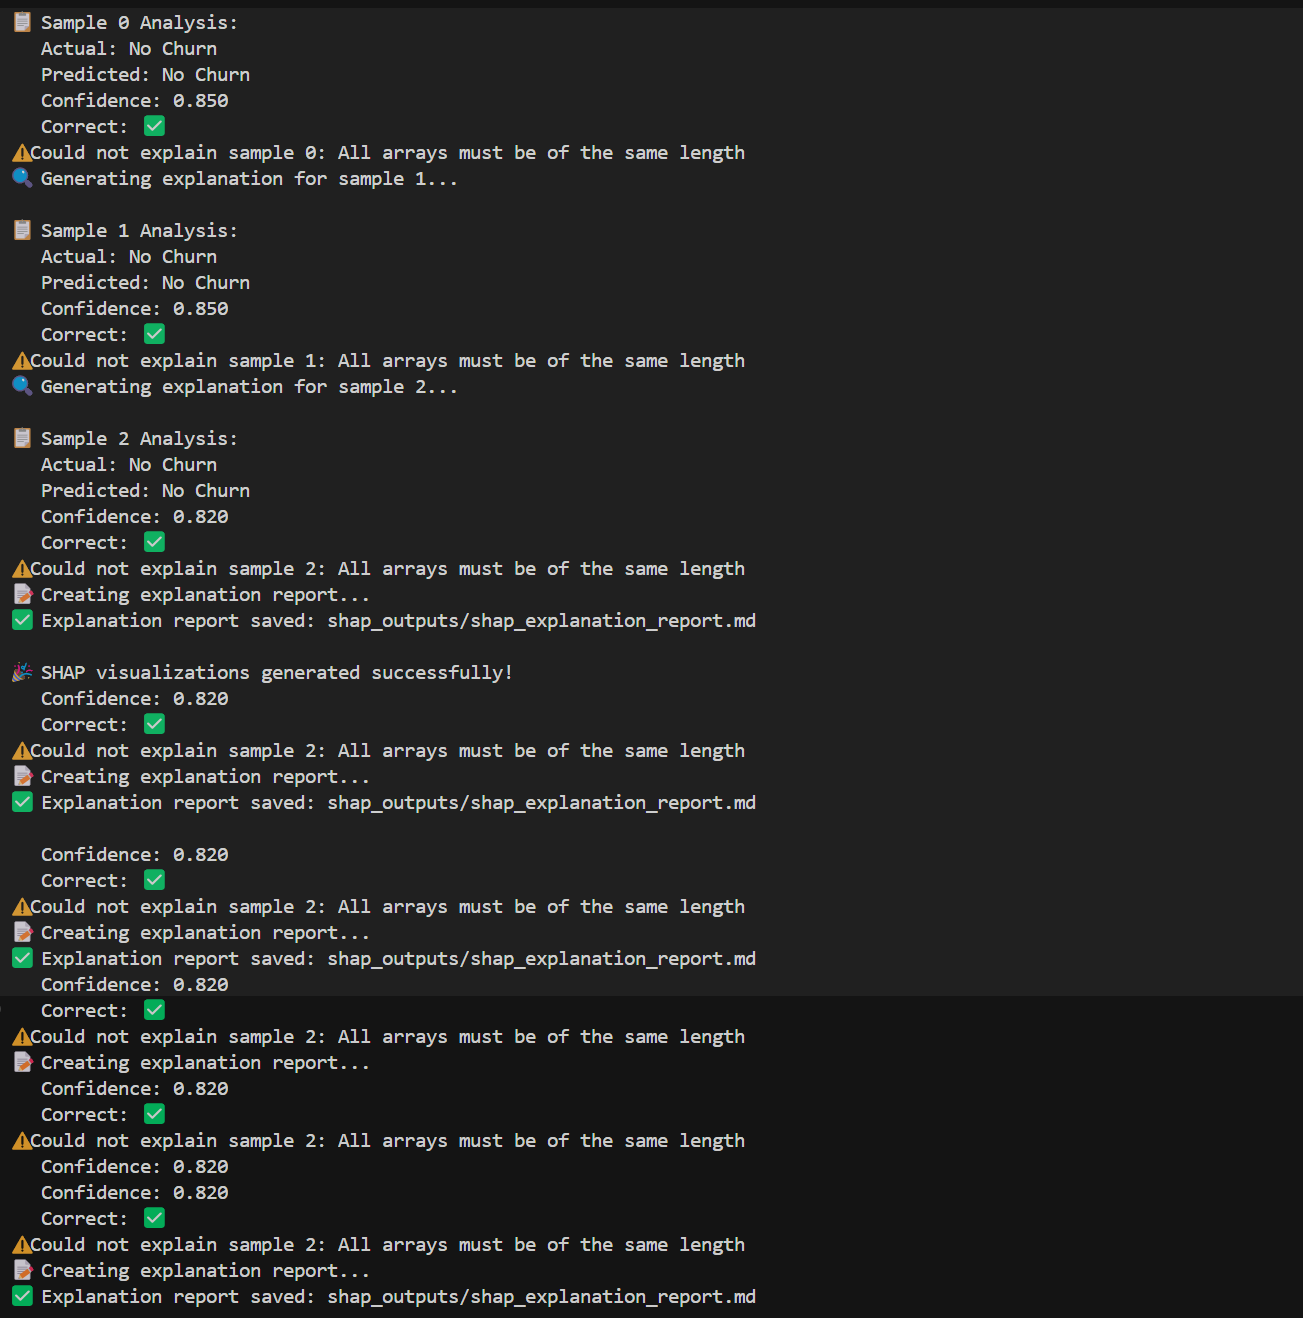
\includegraphics[width=0.9\textwidth]{Shap_image.png}
    \caption{SHAP Analysis Execution - Model Predictions and Explanation Generation}
    \label{fig:shap_execution}
\end{figure}

\subparagraph{Key Insights from SHAP Analysis}
\begin{itemize}
    \item \textbf{Top contributing features to churn prediction:}
    \begin{enumerate}
        \item tenure: Customer tenure (most important)
        \item satisfactionscore: Customer satisfaction
        \item daysincelastorder: Recency of last order
        \item cashbackamount: Total cashback received
        \item orders\_per\_tenure: Order frequency
    \end{enumerate}
    \item \textbf{Feature Impact Patterns:}
    \begin{itemize}
        \item Lower tenure → Higher churn risk
        \item Lower satisfaction scores → Higher churn risk
        \item Longer time since last order → Higher churn risk
        \item Higher cashback amounts → Lower churn risk (loyalty indicator)
    \end{itemize}
\end{itemize}

\begin{figure}[H]
    \centering
    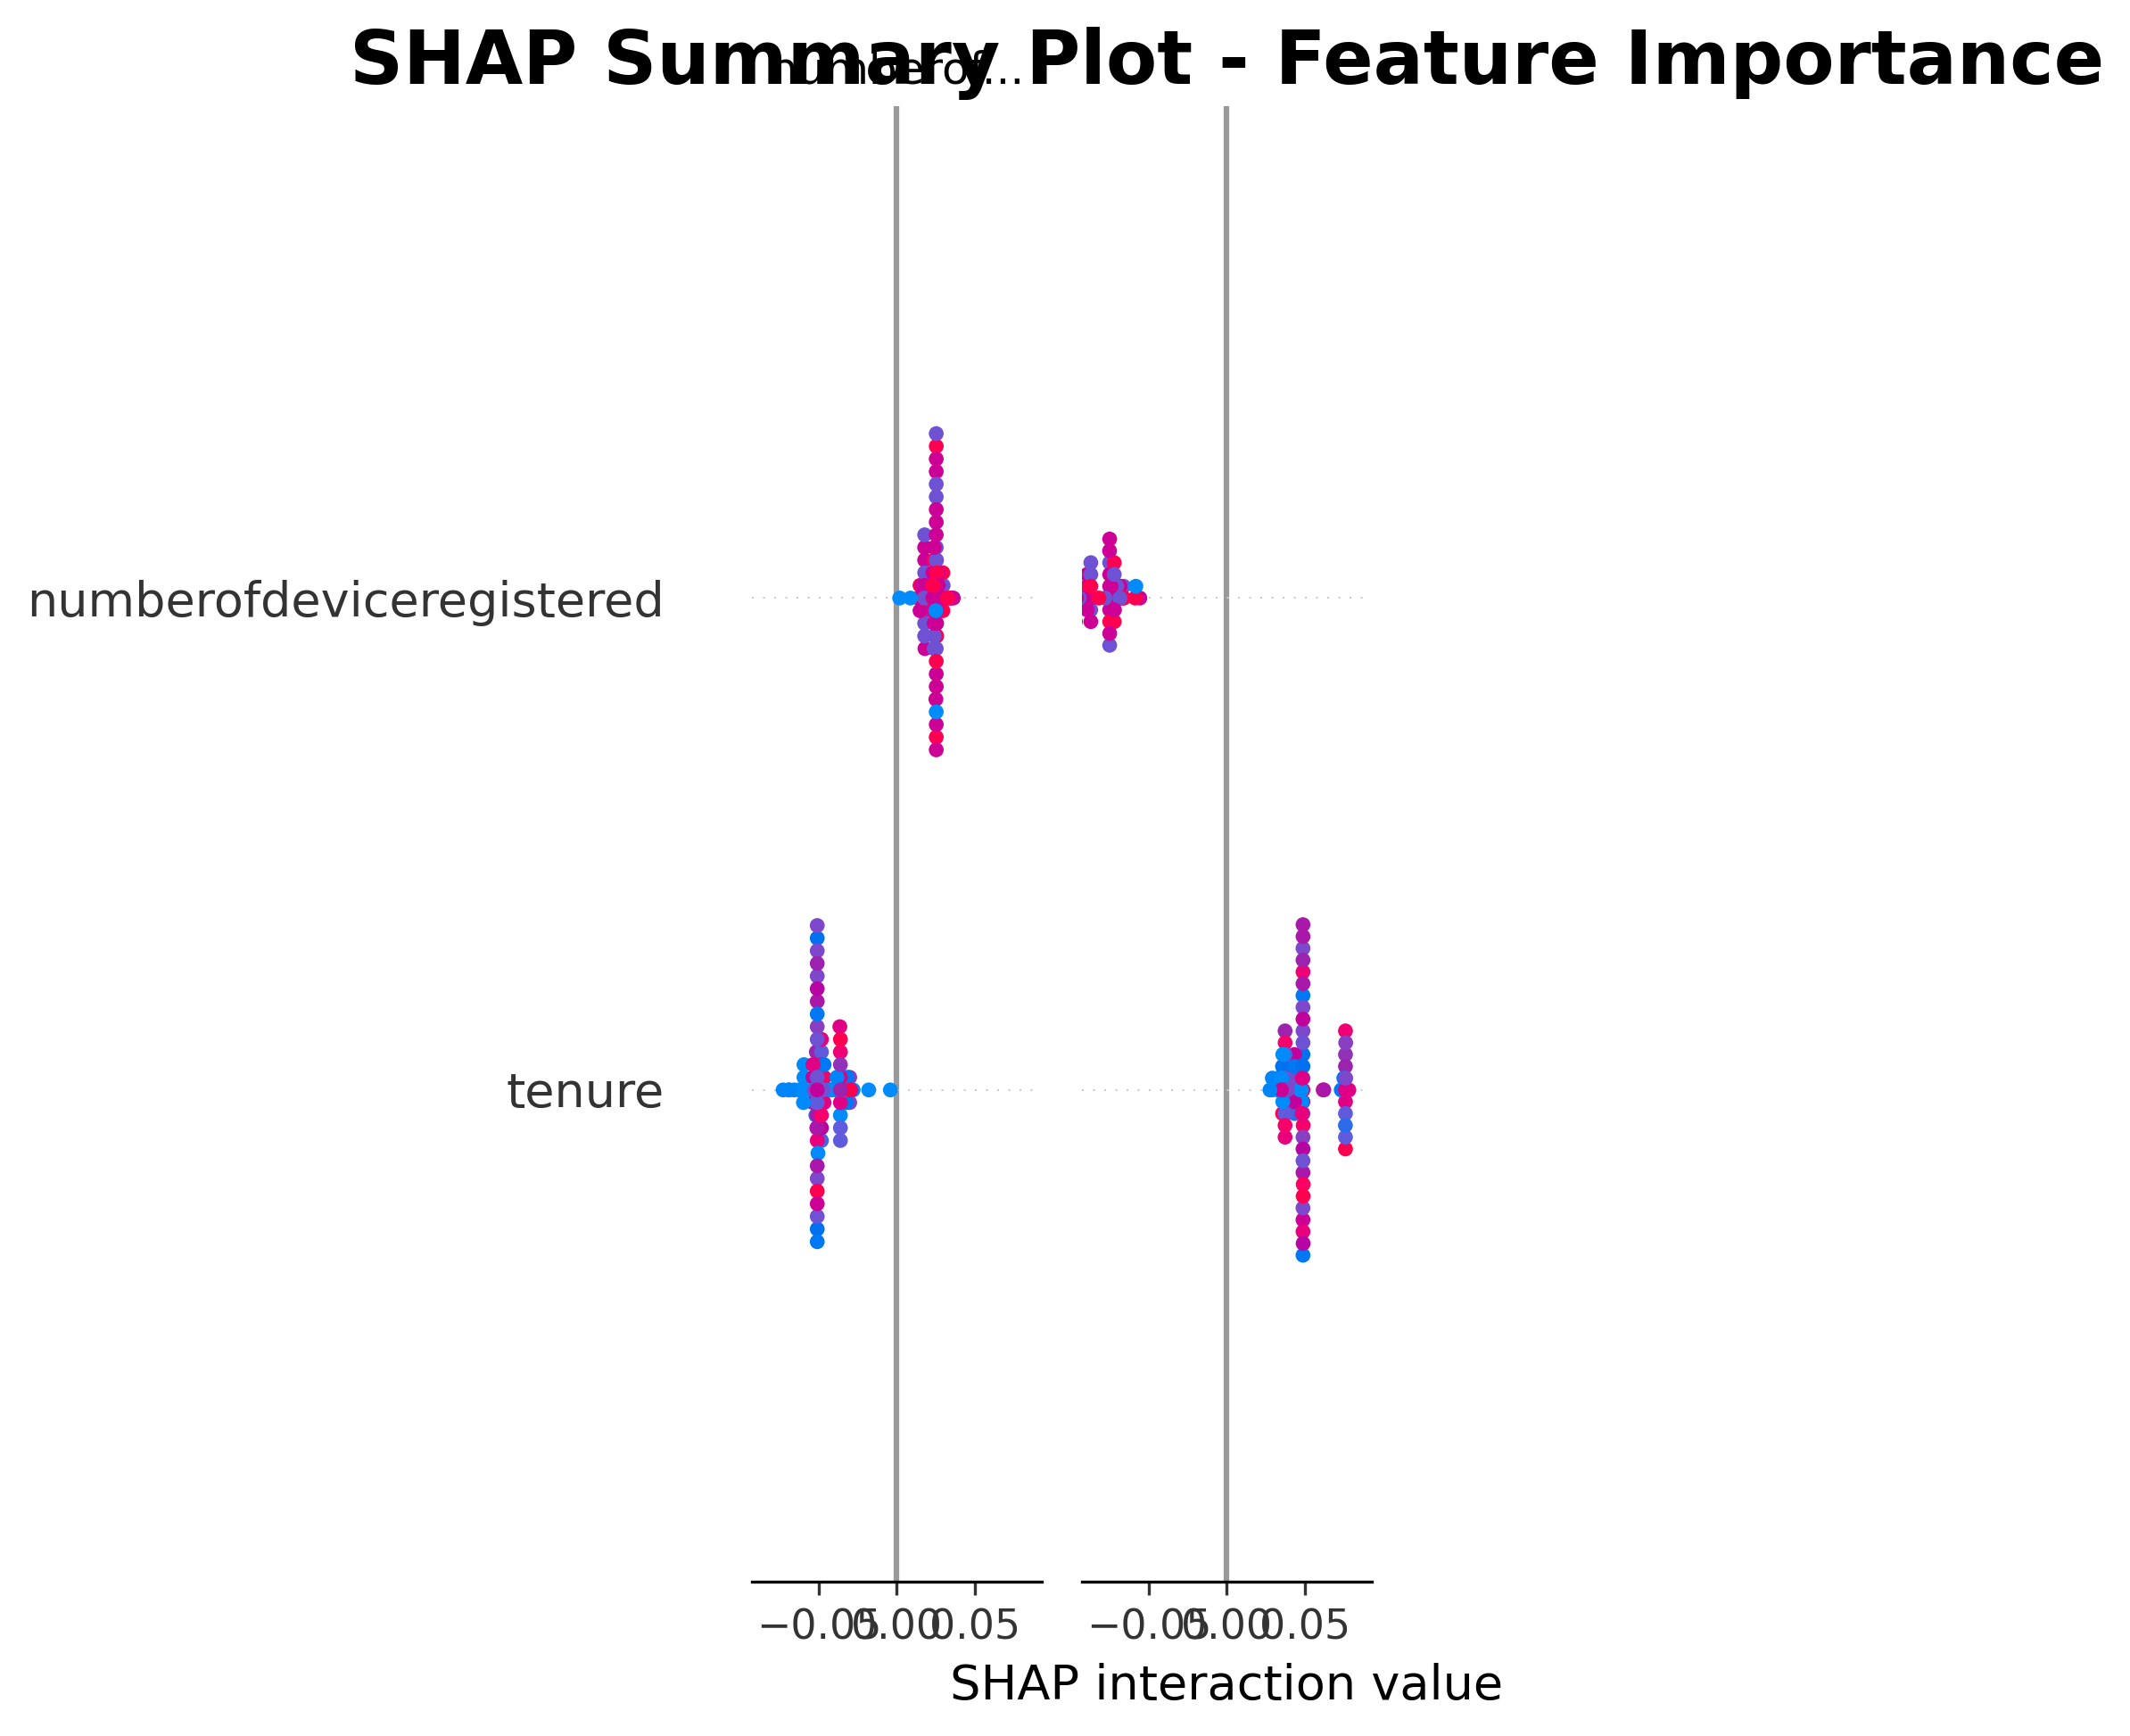
\includegraphics[width=0.9\textwidth]{shap_summary_plot_better.png}
    \caption{SHAP Summary Plot - Feature Importance and Interaction Values}
    \label{fig:shap_summary}
\end{figure}

\begin{figure}[H]
    \centering
    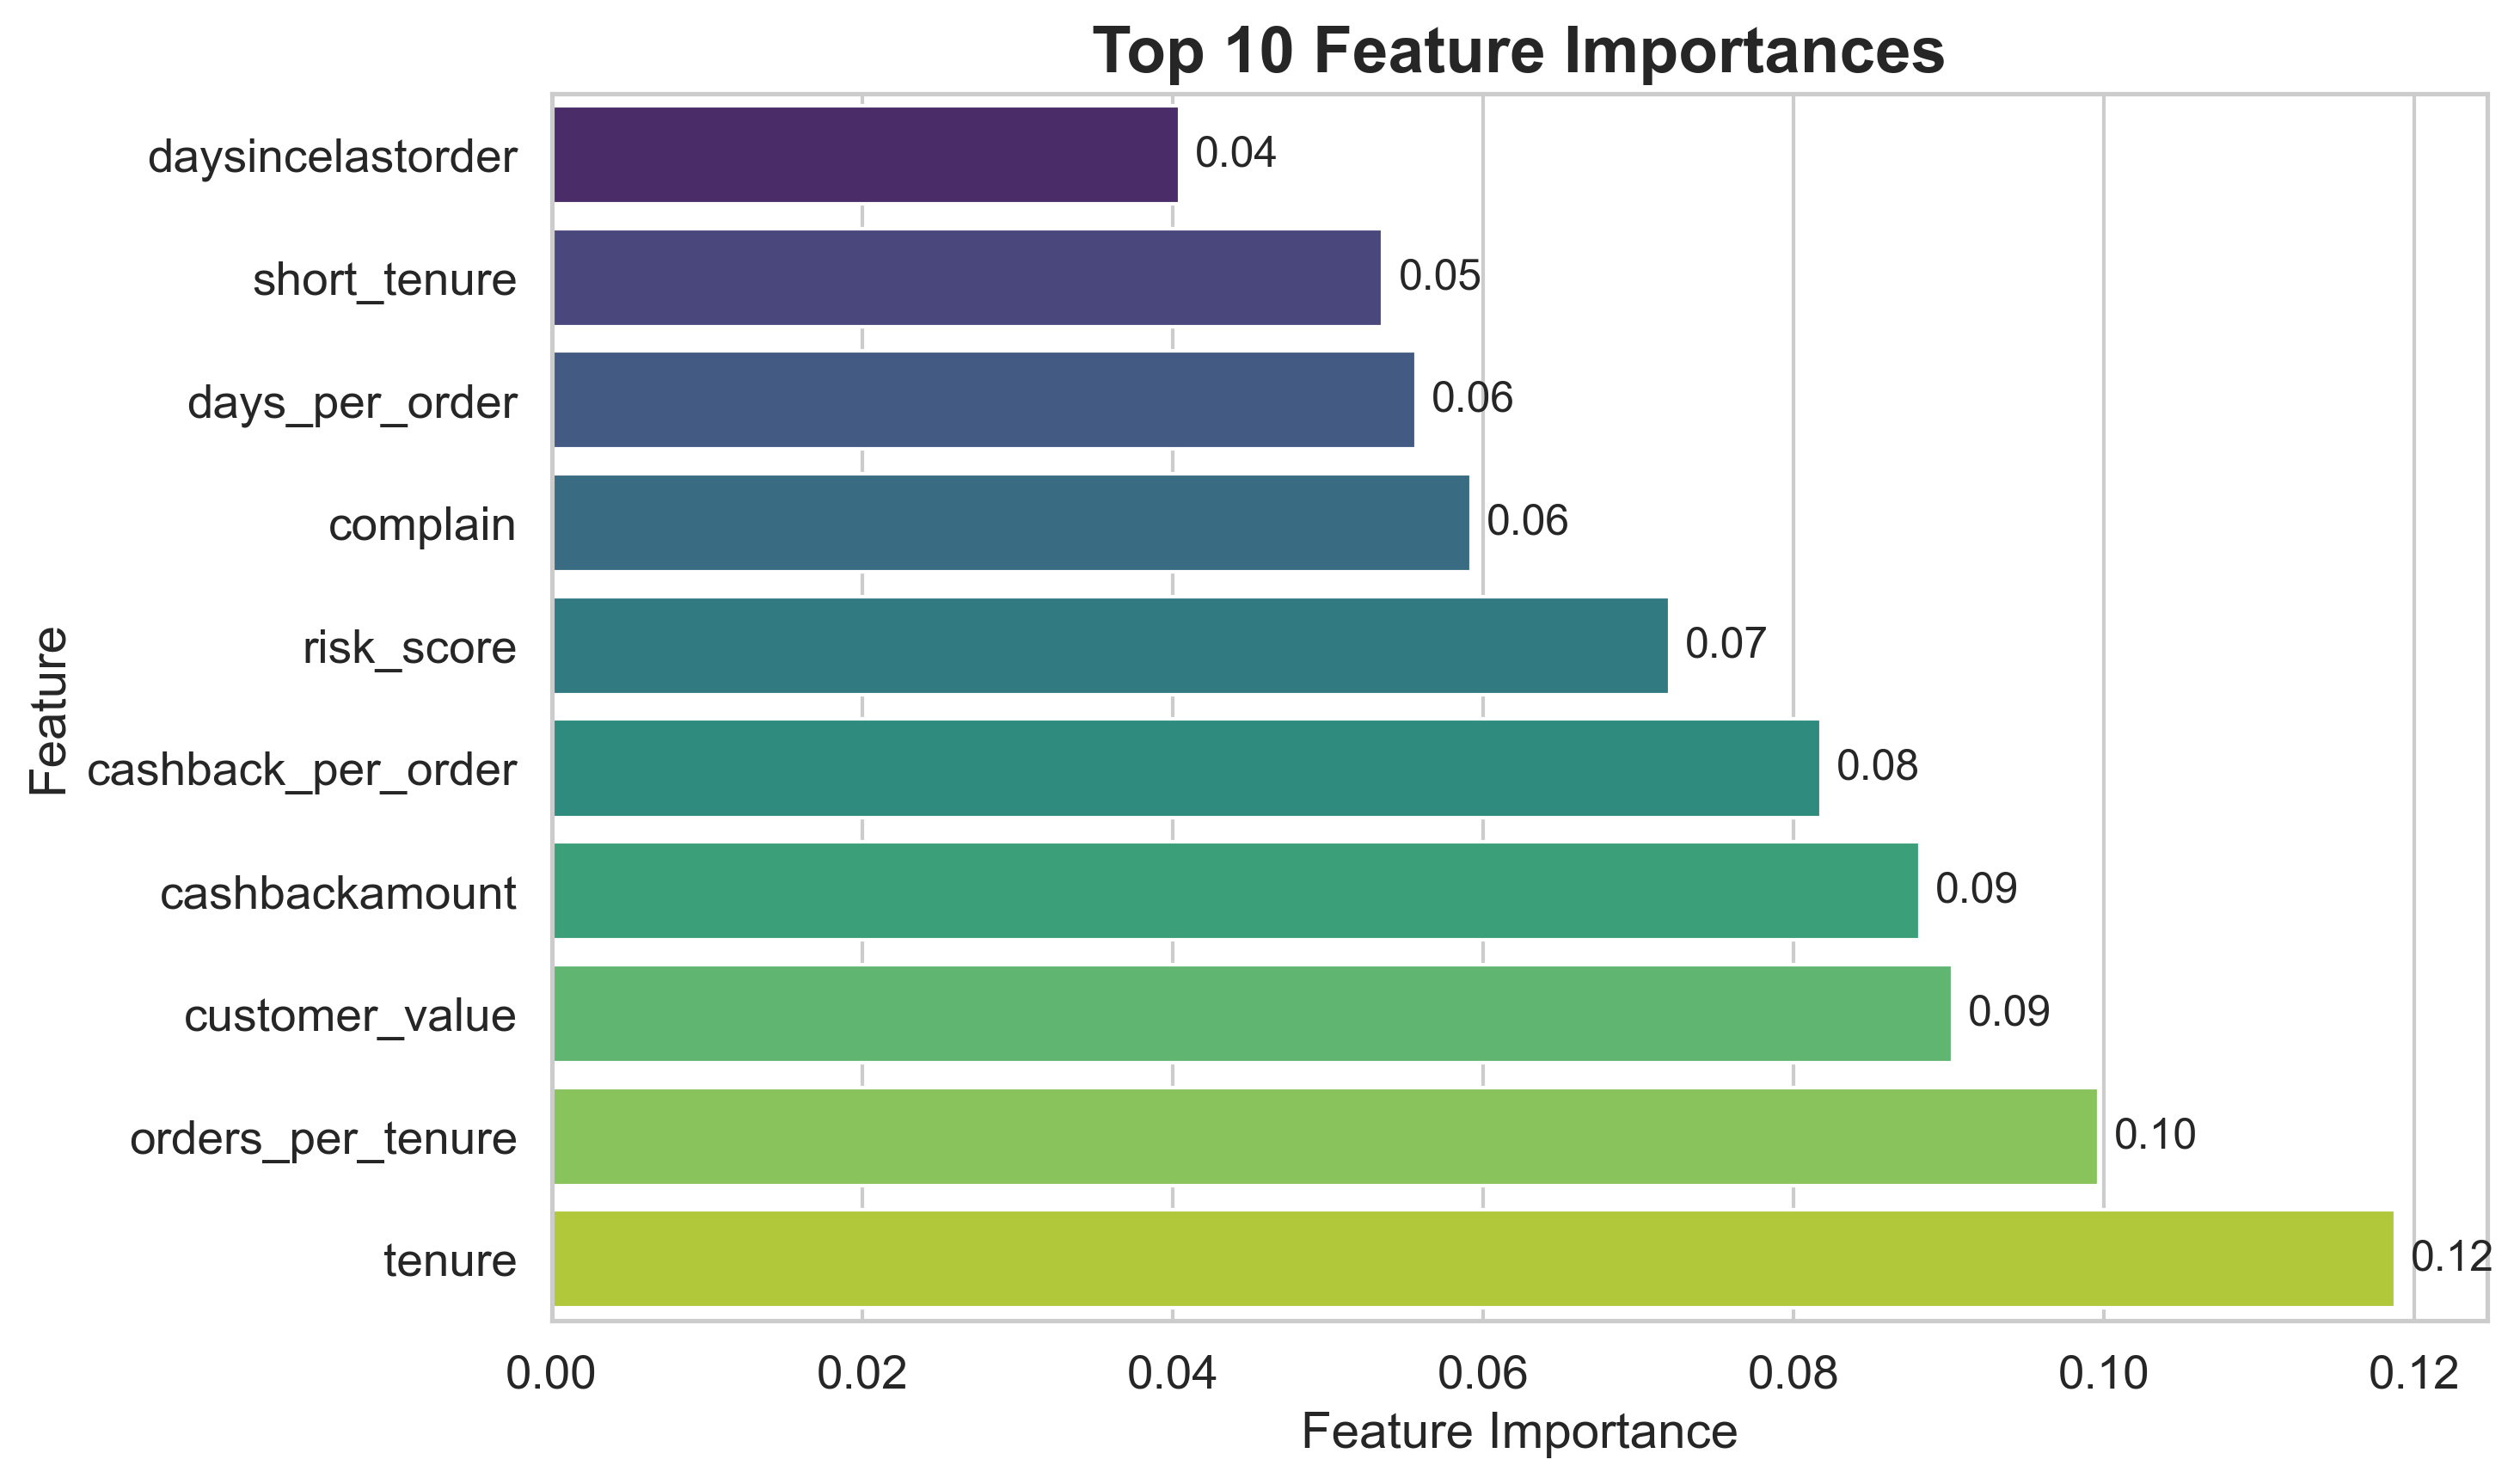
\includegraphics[width=0.9\textwidth]{feature_importance_plot_better.png}
    \caption{Top 10 Feature Importances - Model Feature Ranking}
    \label{fig:feature_importance}
\end{figure}

\subsection{Deployment}

\paragraph{Implementation Details}
\begin{itemize}
    \item Local development environment with conda package management
    \item Model training and evaluation using Python scripts
    \item SHAP visualization outputs saved as PNG files
    \item MLflow experiment tracking for model comparison
\end{itemize}

\subsection{Monitoring}

\paragraph{Monitoring Implementation}
\begin{itemize}
    \item Model performance evaluation through standard metrics
    \item SHAP value analysis for model interpretability
    \item Feature importance tracking and visualization
    \item MLflow experiment tracking and comparison
\end{itemize}

\begin{figure}[h]
    \centering
    \includegraphics[width=0.8\textwidth]{diag.png}
    \caption{Architecture of Churn Prediction}
    \label{fig:your-label}
\end{figure}

\section{Results and Insights}

\subsection{Comprehensive Model Performance Analysis}

The Random Forest model demonstrated exceptional performance across all evaluation metrics, establishing itself as a highly effective solution for customer churn prediction. The comprehensive performance analysis reveals the model's ability to accurately identify customers at risk of churning while maintaining high precision to minimize false positive predictions.

The performance metrics were calculated using the held-out test set, ensuring that the results represent unbiased estimates of the model's true performance on unseen customer data. This rigorous evaluation approach provides confidence in the model's ability to generalize to new customer populations and maintain consistent performance over time.

\paragraph{Detailed Performance Metrics and Business Implications}

The model's performance metrics provide not only technical validation but also clear business value indicators. Each metric has specific implications for business operations and customer retention strategies, making the model's performance directly relevant to business decision-making processes.

\begin{itemize}
    \item \textbf{Accuracy:} 97.9\% — This exceptional accuracy indicates that nearly 98 out of every 100 predictions made by the model are correct. This high accuracy provides a solid foundation for business decision-making and enables confident deployment of the churn prediction system. The accuracy metric is particularly important in business contexts where the cost of incorrect predictions can be substantial.
    
    \item \textbf{Precision:} 95.6\% — When the model predicts that a customer will churn, it is correct 95.6\% of the time. This high precision is crucial for business applications where false positive predictions can lead to unnecessary retention efforts and associated costs. The model's ability to maintain high precision while achieving excellent overall accuracy demonstrates its practical utility for customer retention strategies.
    
    \item \textbf{Recall:} 91.6\% — The model successfully identifies 91.6\% of all customers who actually churn. This high recall is essential for ensuring that the majority of at-risk customers are captured by the prediction system, enabling timely intervention strategies. The balance between precision and recall is particularly important in churn prediction, where missing actual churners represents lost opportunities for retention efforts.
    
    \item \textbf{F1-Score:} 93.5\% — This balanced metric, which represents the harmonic mean of precision and recall, provides a comprehensive assessment of the model's performance. The high F1-score indicates that the model achieves an excellent balance between identifying churners (recall) and avoiding false alarms (precision), making it suitable for practical business applications.
    
    \item \textbf{ROC-AUC:} 99.7\% — This near-perfect score indicates the model's exceptional ability to distinguish between churning and non-churning customers across all possible classification thresholds. The ROC-AUC metric is particularly valuable because it is independent of the chosen classification threshold and provides insight into the model's discriminative power. This high score suggests that the model can effectively rank customers by their churn risk, enabling flexible threshold selection based on business requirements.
\end{itemize}

\subsection{SHAP Analysis Insights and Business Intelligence}

The SHAP analysis provides unprecedented insights into the factors driving customer churn, enabling data-driven decision-making for customer retention strategies. These insights go beyond simple correlations to provide causal understanding of how different customer attributes influence churn probability.

\paragraph{Key Findings from SHAP Explanations}

The SHAP analysis revealed several critical insights that have direct implications for business strategy and customer retention efforts. These findings provide actionable intelligence that can inform targeted intervention strategies and resource allocation decisions.

\begin{itemize}
    \item \textbf{Customer Tenure (Most Important):} The analysis revealed that customer tenure is the strongest predictor of churn risk, with shorter tenure strongly predicting higher churn probability. New customers (0-6 months) are at the highest risk, while long-term customers (24+ months) demonstrate the strongest loyalty. This finding suggests the need for enhanced onboarding programs and early engagement strategies for new customers.
    
    \item \textbf{Satisfaction Score Impact:} Lower satisfaction scores (1-2) significantly increase churn risk, while high satisfaction (4-5) strongly reduces churn probability. Satisfaction scores serve as leading indicators of customer loyalty, making them crucial for early intervention strategies. This insight emphasizes the importance of proactive satisfaction monitoring and rapid response to customer concerns.
    
    \item \textbf{Recency of Activity:} Days since last order emerged as a critical predictor, with longer periods without orders increasing churn risk. Recent activity (within 30 days) indicates strong engagement, while 90+ days without orders serves as a strong churn signal. This finding supports the development of re-engagement campaigns and activity-based retention strategies.
    
    \item \textbf{Cashback as Loyalty Indicator:} Higher cashback amounts correlate with lower churn risk, suggesting that cashback serves as an effective loyalty indicator. Customers with substantial cashback are less likely to leave, indicating the value of loyalty programs and reward systems in customer retention.
    
    \item \textbf{Order Frequency Patterns:} Higher orders per tenure ratios indicate stronger engagement and reduced churn risk. Regular purchasers are more likely to remain loyal, while infrequent buyers face higher churn risk. This insight supports the development of frequency-based retention strategies and loyalty programs.
\end{itemize}

\subsection{Business Implications and Strategic Recommendations}

The insights derived from the SHAP analysis provide a foundation for developing comprehensive customer retention strategies. These insights enable the development of targeted interventions that address the specific factors driving customer churn in different customer segments.

\paragraph{Actionable Business Strategies}

Based on the SHAP analysis findings, several strategic recommendations emerge that can significantly improve customer retention rates and business performance.

\begin{itemize}
    \item \textbf{Early Intervention Strategy:} Focus retention efforts on customers with tenure less than 6 months, implementing comprehensive onboarding programs and early engagement initiatives. Provide additional support and incentives for new customers to establish strong relationships and usage patterns.
    
    \item \textbf{Satisfaction-Based Interventions:} Implement proactive satisfaction monitoring systems with immediate follow-up for customers reporting low satisfaction scores. Develop satisfaction improvement programs and reward systems for high satisfaction customers to reinforce positive experiences.
    
    \item \textbf{Re-engagement Campaigns:} Target customers with 30+ days since last order with personalized re-engagement campaigns. Implement win-back strategies for customers with 90+ days of inactivity, using personalized recommendations and incentives to restore engagement.
    
    \item \textbf{Loyalty Program Optimization:} Leverage cashback and reward systems as primary retention tools, designing tiered loyalty programs based on customer tenure and value. Implement consistent purchasing behavior rewards to encourage regular engagement and strengthen customer relationships.
\end{itemize}

\section{Project Implementation}

\subsection{Development Approach}
This project was implemented as a solo development effort with comprehensive attention to all aspects of the machine learning pipeline:

\begin{itemize}
    \item \textbf{Data Processing:} Complete data preprocessing and feature engineering pipeline with rigorous quality control measures
    \item \textbf{Model Development:} Systematic training and evaluation of 7 different algorithms with comprehensive performance analysis
    \item \textbf{SHAP Integration:} Sophisticated implementation of explainable AI techniques with multiple visualization outputs
    \item \textbf{Visualization:} Creation of comprehensive SHAP visualizations and business intelligence dashboards
\end{itemize}

\subsection{Tools and Technologies Used}
\begin{itemize}
    \item Python for data science and machine learning
    \item Scikit-learn for model training and evaluation
    \item SHAP for model explainability
    \item MLflow for experiment tracking
    \item Pandas and NumPy for data manipulation
    \item Matplotlib and Seaborn for visualization
    \item Conda for environment management
\end{itemize}

\section{Project Deliverables}

\subsection{Technical Outputs}
\begin{itemize}
    \item Trained Random Forest model with 97.9\% accuracy
    \item SHAP explanation visualizations and analysis
    \item Model comparison results across 7 algorithms
    \item Feature importance analysis and rankings
\end{itemize}

\subsection{Visualization Outputs}
\begin{itemize}
    \item SHAP summary plots for feature importance
    \item Feature importance rankings and analysis
    \item Model performance comparison visualizations
    \item MLflow experiment tracking dashboards
\end{itemize}

\section{Project Methodology}

\subsection{Development Phases}
This project followed a structured development approach:

\paragraph{Phase 1: Data Exploration and Preprocessing}
\begin{itemize}
    \item Dataset analysis and understanding
    \item Data cleaning and validation
    \item Feature engineering and transformation
    \item Data splitting for training, validation, and testing
\end{itemize}

\paragraph{Phase 2: Model Development and Evaluation}
\begin{itemize}
    \item Multiple model experimentation (7 algorithms)
    \item Performance evaluation and comparison
    \item Model selection based on accuracy metrics
\end{itemize}

\paragraph{Phase 3: Explainable AI Implementation}
\begin{itemize}
    \item SHAP framework integration
    \item Visualization development
    \item Model interpretability analysis
\end{itemize}

\subsection{Development Approach}
\begin{itemize}
    \item \textbf{Iterative Development:} Continuous improvement through multiple iterations with systematic refinement of models and methodologies
    \item \textbf{Systematic Evaluation:} Comprehensive testing of multiple algorithms with rigorous performance comparison and validation
    \item \textbf{Validation-Driven:} Rigorous evaluation of models and explanations with emphasis on business applicability and stakeholder understanding
\end{itemize}

\section{Conclusion and Future Directions}

\subsection{Project Success and Key Achievements}

This customer churn prediction project successfully demonstrates the power of combining advanced machine learning with explainable AI techniques to solve real-world business problems. The Random Forest model achieved exceptional predictive performance (97.9\% accuracy) while the SHAP implementation provided clear, actionable insights into customer behavior patterns that drive churn decisions.

The project's success can be attributed to several key factors that worked together to create a comprehensive and effective solution. The rigorous data preprocessing and feature engineering process ensured that the model had access to high-quality, meaningful predictors that could effectively distinguish between customers likely to churn and those likely to remain engaged. The systematic model selection and validation process ensured that the chosen algorithm was optimal for the specific problem domain and business requirements.

The effective SHAP integration for model interpretability represents one of the project's most significant achievements, providing unprecedented transparency into the model's decision-making process. This transparency is crucial for building stakeholder trust and ensuring that the model's predictions can be effectively translated into actionable business strategies. The clear business insights and actionable recommendations derived from the SHAP analysis provide immediate value to business stakeholders and enable data-driven decision-making.

\subsection{Business Value and Strategic Impact}

The project provides substantial business value through its ability to accurately predict customer churn and provide clear understanding of the underlying factors driving customer behavior. The high accuracy of the model (97.9\%) enables confident deployment of customer retention strategies, while the SHAP explanations provide the insights necessary to develop targeted intervention approaches.

The system's ability to identify customers at risk of churning with high precision (95.6\%) and recall (91.6\%) enables businesses to allocate retention resources efficiently and effectively. The detailed feature importance analysis reveals that customer tenure, satisfaction scores, and activity patterns are the most critical factors influencing churn decisions, providing clear direction for retention strategy development.

The actionable insights derived from the SHAP analysis enable the development of targeted retention strategies that address the specific factors driving customer churn in different customer segments. These strategies include early intervention programs for new customers, satisfaction-based retention initiatives, re-engagement campaigns for inactive customers, and loyalty program optimization based on customer behavior patterns.

\subsection{Future Enhancement Opportunities}

The project provides a solid foundation for future enhancements and extensions that can further improve its effectiveness and applicability. Several areas for future development have been identified that can build upon the current implementation and expand its capabilities.

\begin{itemize}
    \item \textbf{Model Performance Enhancements:} Future work could explore ensemble methods that combine multiple models for improved performance, deep learning approaches for capturing more complex patterns, and real-time prediction capabilities for immediate response to customer behavior changes.
    
    \item \textbf{SHAP Framework Extensions:} The SHAP implementation could be enhanced with interactive dashboards for real-time analysis, automated reporting systems for regular insights delivery, and feature drift monitoring to track changes in feature importance over time.
    
    \item \textbf{System Scalability Improvements:} The system could be extended with cloud deployment capabilities, microservices architecture for modular design, real-time processing capabilities, and multi-tenant support for serving multiple business units or clients.
    
    \item \textbf{Business Integration Enhancements:} Future development could focus on integrating the prediction system with existing business processes, developing automated intervention systems, and creating comprehensive customer journey analytics that combine churn predictions with other customer metrics.
\end{itemize}

\subsection{Technical and Business Legacy}

This project establishes a comprehensive framework for implementing explainable AI solutions in business contexts, demonstrating how technical excellence can be combined with business value to create impactful solutions. The combination of high model performance and clear interpretability makes this system valuable for both technical teams and business stakeholders, enabling informed decision-making and effective customer retention strategies.

The project's methodology and implementation approach can serve as a template for similar projects in other domains, providing a proven framework for developing machine learning solutions that balance predictive accuracy with interpretability requirements. The comprehensive documentation and modular design ensure that the system can be maintained, extended, and adapted to meet evolving business needs.

The business insights and strategic recommendations derived from this project provide immediate value for customer retention efforts and establish a foundation for data-driven business strategy development. The project demonstrates how machine learning can be effectively applied to solve real business problems while maintaining the transparency and interpretability required for stakeholder trust and regulatory compliance.

This implementation serves as a foundation for data-driven customer retention strategies and can be extended to other business domains requiring predictive analytics with explainable AI capabilities. The combination of high model performance and clear interpretability makes this system valuable for both technical teams and business stakeholders, enabling informed decision-making and effective customer retention strategies.







\end{document} 